
\chapter{Matrix Transpose}

The Matrix transpose is an operation where the columns of the matrix 
and the rows of the matrix interchanged. This operation also affects 
the matrix layout; if the matrix is a Column-Major, then after the 
transpose, it will be the Row-Major and vice-versa. The transpose 
operation is an involution (self-inverse) operation for the matrix or the vector.


\[
A= 
\begin{bmatrix}
    a_{00}  & a_{01}    & \dots     & a_{0k}\\
    a_{10}  & a_{11}    & \dots     & a_{1k}\\
    \vdots  & \vdots    & \ddots    & \vdots\\
    a_{m0}  & a_{m1}    & \dots     & a_{mk}\\
\end{bmatrix}
\]

\vspace*{0.5cm}


\[
C = A^T
\]

\[
\begin{bmatrix}
    c_{00}  & c_{01}    & \dots     & c_{0n}\\
    c_{10}  & c_{11}    & \dots     & c_{1n}\\
    \vdots  & \vdots    & \ddots    & \vdots\\
    c_{m0}  & c_{m1}    & \dots     & c_{mn}\\
\end{bmatrix}
= 
\begin{bmatrix}
    a_{00}  & a_{10}    & \dots     & a_{m0}\\
    a_{01}  & a_{11}    & \dots     & a_{m1}\\
    \vdots  & \vdots    & \ddots    & \vdots\\
    a_{0k}  & a_{1k}    & \dots     & a_{mk}\\
\end{bmatrix}
\]

\vspace*{0.5cm}

Involution Property: $(A^T)^T = A$

\clearpage

\section{Algorithm}

We divide the matrix into smaller blocks to optimise the transpose 
operation to keep the block inside the L1 cache and increase the 
cache hit. For the in-place algorithm, we use the fact that the 
matrix is symmetrical around the diagonal, which reduces the cost 
of bringing the other block matrix when we can swap the entries 
around the diagonal. This fact is valid for the block which is 
on the diagonal but for the other blocks, and we simply swap 
every with the corresponding block.

\subsection{Out-Of-Place Transpose}

\begin{figure}[htb]
    \centering
    \caption*{Block Diagram for Out-Of-Place Transpose}
    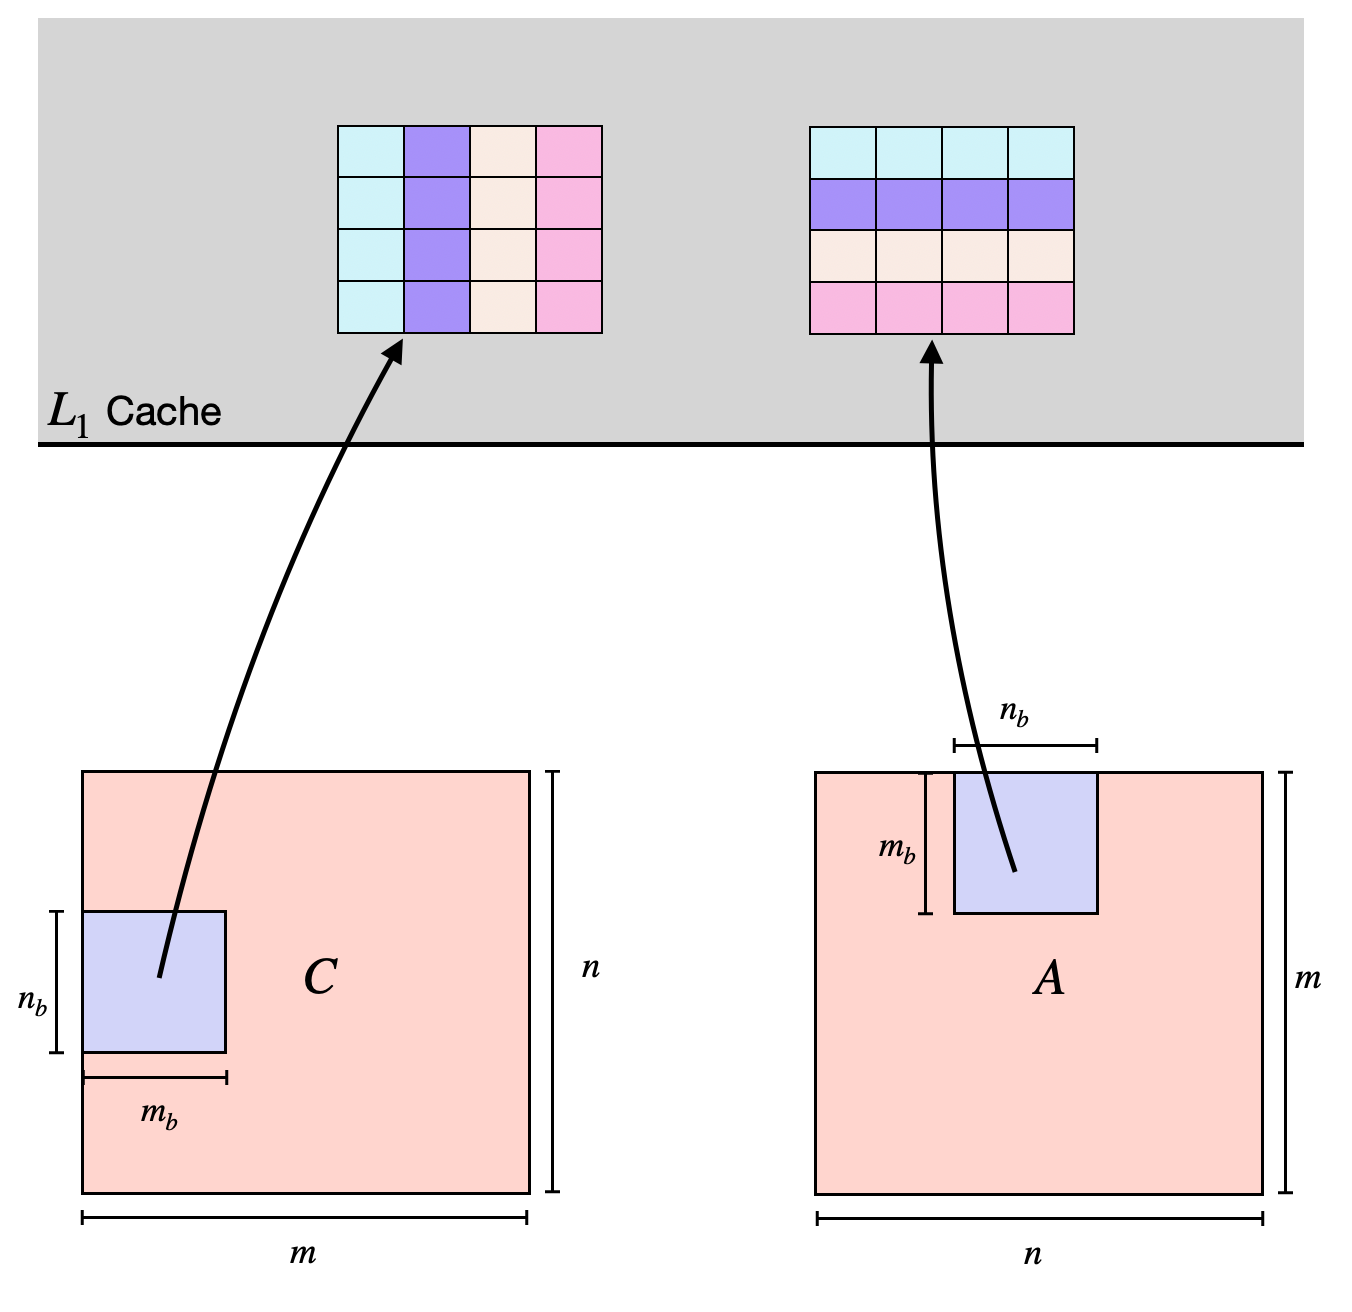
\includegraphics[width=8cm]{../assets/transpose/outplace/outplace_trans.png}%
\end{figure}

\begin{algorithm}[H]
    \SetAlgoLined
    \SetKwFunction{SIMDFn}{$simd\_loop$}
    \SetKwProg{Fn}{Function}{:}{end}

    \tcp{$c$    is the pointer to the output Matrix}
    \tcp{$wc$   is the pointer to the strides of the output Matrix}
    \tcp{$a$    is the pointer to the input Matrix $A$}
    \tcp{$wa$   is the pointer to the strides of the input Matrix $A$}
    \tcp{$m$    is the row-block of the Matrix $A$}
    \tcp{$n$    is the col-block of the Matrix $A$}
    \Fn{\SIMDFn($c$, $wc$, $a$, $wa$, $m$, $n$)}{

        \For{\assign{i}{0} \KwTo $m$ \KwBy $1$}{
            \assignln{cj}{c + wc[1] \times i}
            \assignln{aj}{a + wa[0] \times i}
            \openmp{simd}
            \For{\assign{j}{0} \KwTo $n$ \KwBy $1$}{
                \assignln{cj[wc[0] \times j]}{aj [ wa[1] \times j ]}
            }
        }
    }
    \caption{Out-Of-Place Matrix Transpose SIMD Function}
\end{algorithm}


\begin{algorithm}[H]
    \SetAlgoLined
    \KwIn{$c$, $n_c$, $w_c$ $a$, $n_a$, $w_a$, $num\_threads$}
    \tcp{$c$    is the pointer to the output Matrix}
    \tcp{$n_c$  is pointer to the dimensions of the output Matrix}
    \tcp{$w_c$  is pointer to the strides of the output Matrix}
    \tcp{$a$    is the pointer to the input Matrix}
    \tcp{$n_a$  is pointer to the dimensions of the output Matrix}
    \tcp{$w_a$  is pointer to the strides of the output Matrix}
    \tcp{$num\_threads$ is the user provided thread count}
    \tcp{$block$ is the block size for the simd loop}

    \Begin{
        \assignln{m}{n_a[0]}
        \assignln{n}{n_a[1]}
        \assignln{max\_blocks}{max( 1, \lfloor \frac{ m }{block} \rfloor )}
        \assignln{max\_threads}{min( max\_blocks, num\_threads )}
        \openmp{parallel for num\_threads(max\_threads) schedule(dynamic)}
        \For{\assign{j}{0} \KwTo $m$ \KwBy $block$}{
            \assignln{ib}{min( m - i, block)}
            \assignln{aj}{a + i \times wa[0]}
            \assignln{cj}{c + i \times wc[1]}
            \For{\assign{i}{0} \KwTo $n$ \KwBy $block$}{
                \assignln{jb}{min( n - i, block)}
                \assignln{ak}{a + j \times wa[1]}
                \assignln{ck}{c + j \times wc[0]}
                $simd\_loop(ck, w_c, ak, w_a, ib, jb)$
            }
        }
    }

    \caption{Out-Of-Place Matrix Transpose}
\end{algorithm}

\subsection{In-Place Transpose}

\begin{figure}[htb]
    \centering
    \caption*{Block Diagram for In-Place Transpose}
    \subfloat[\centering Blocks are Different]{{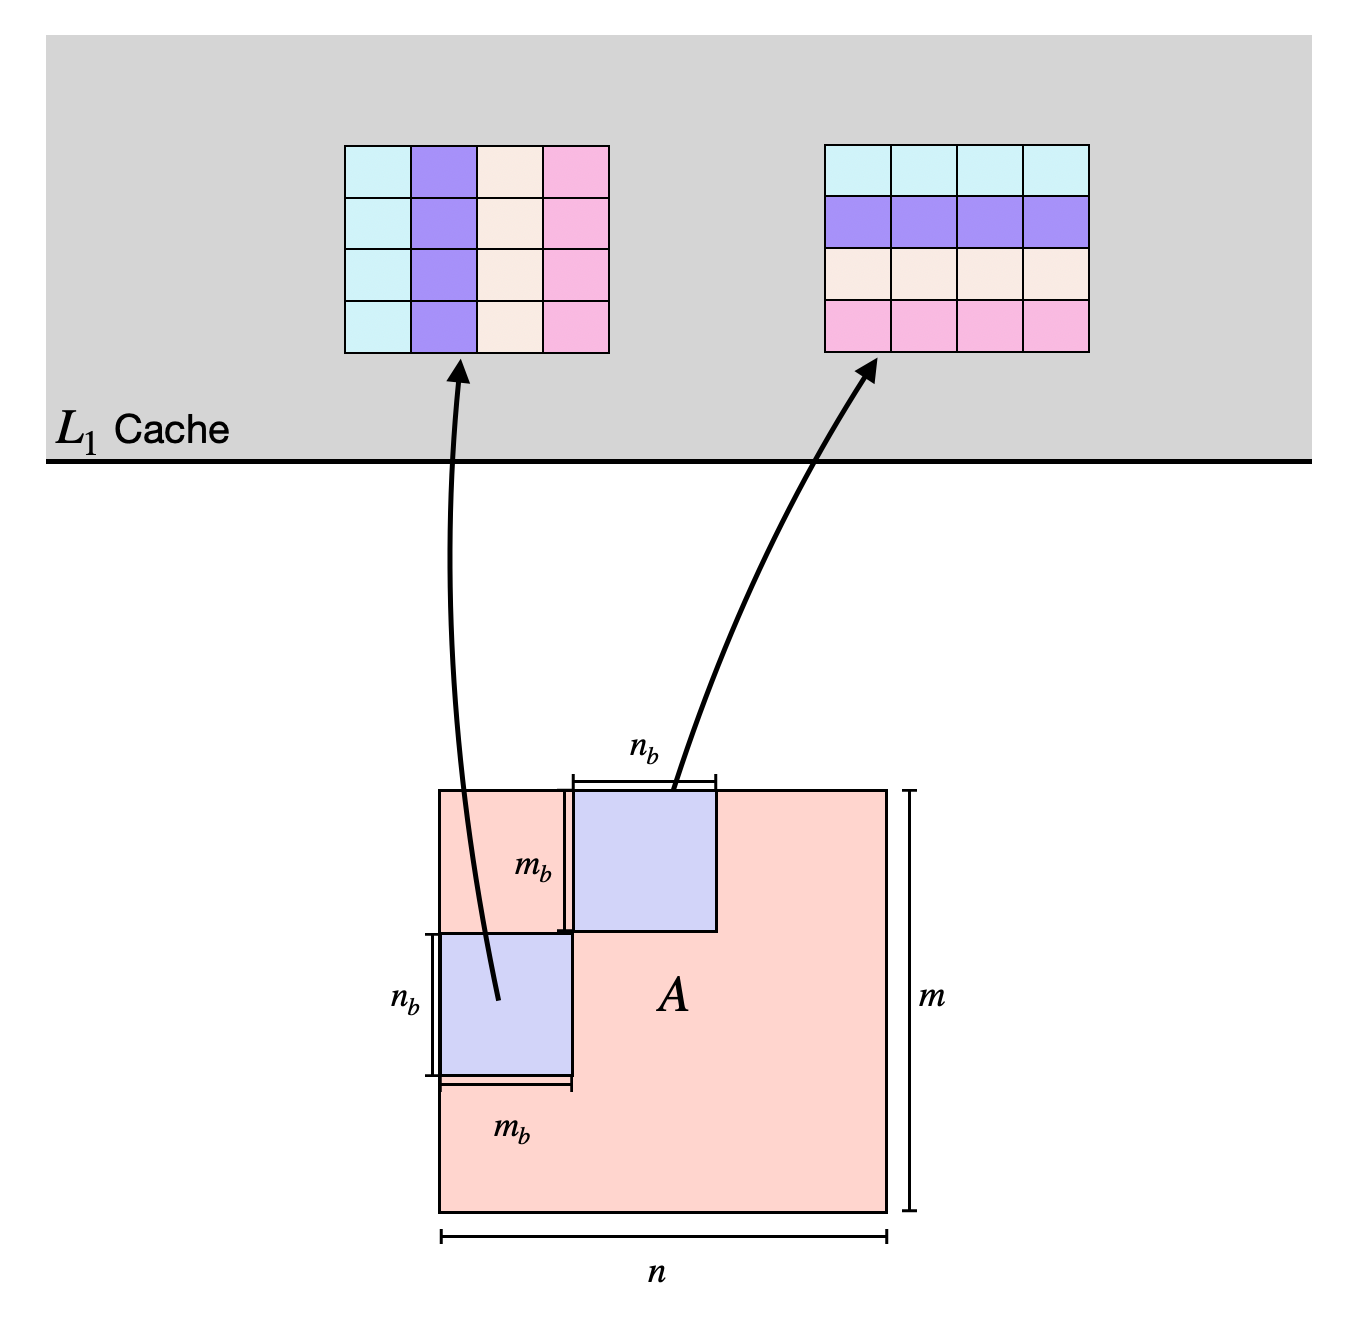
\includegraphics[width=8cm]{../assets/transpose/inplace/inplace_trans1.png} }}%
    \qquad
    \subfloat[\centering Blocks are Same]{{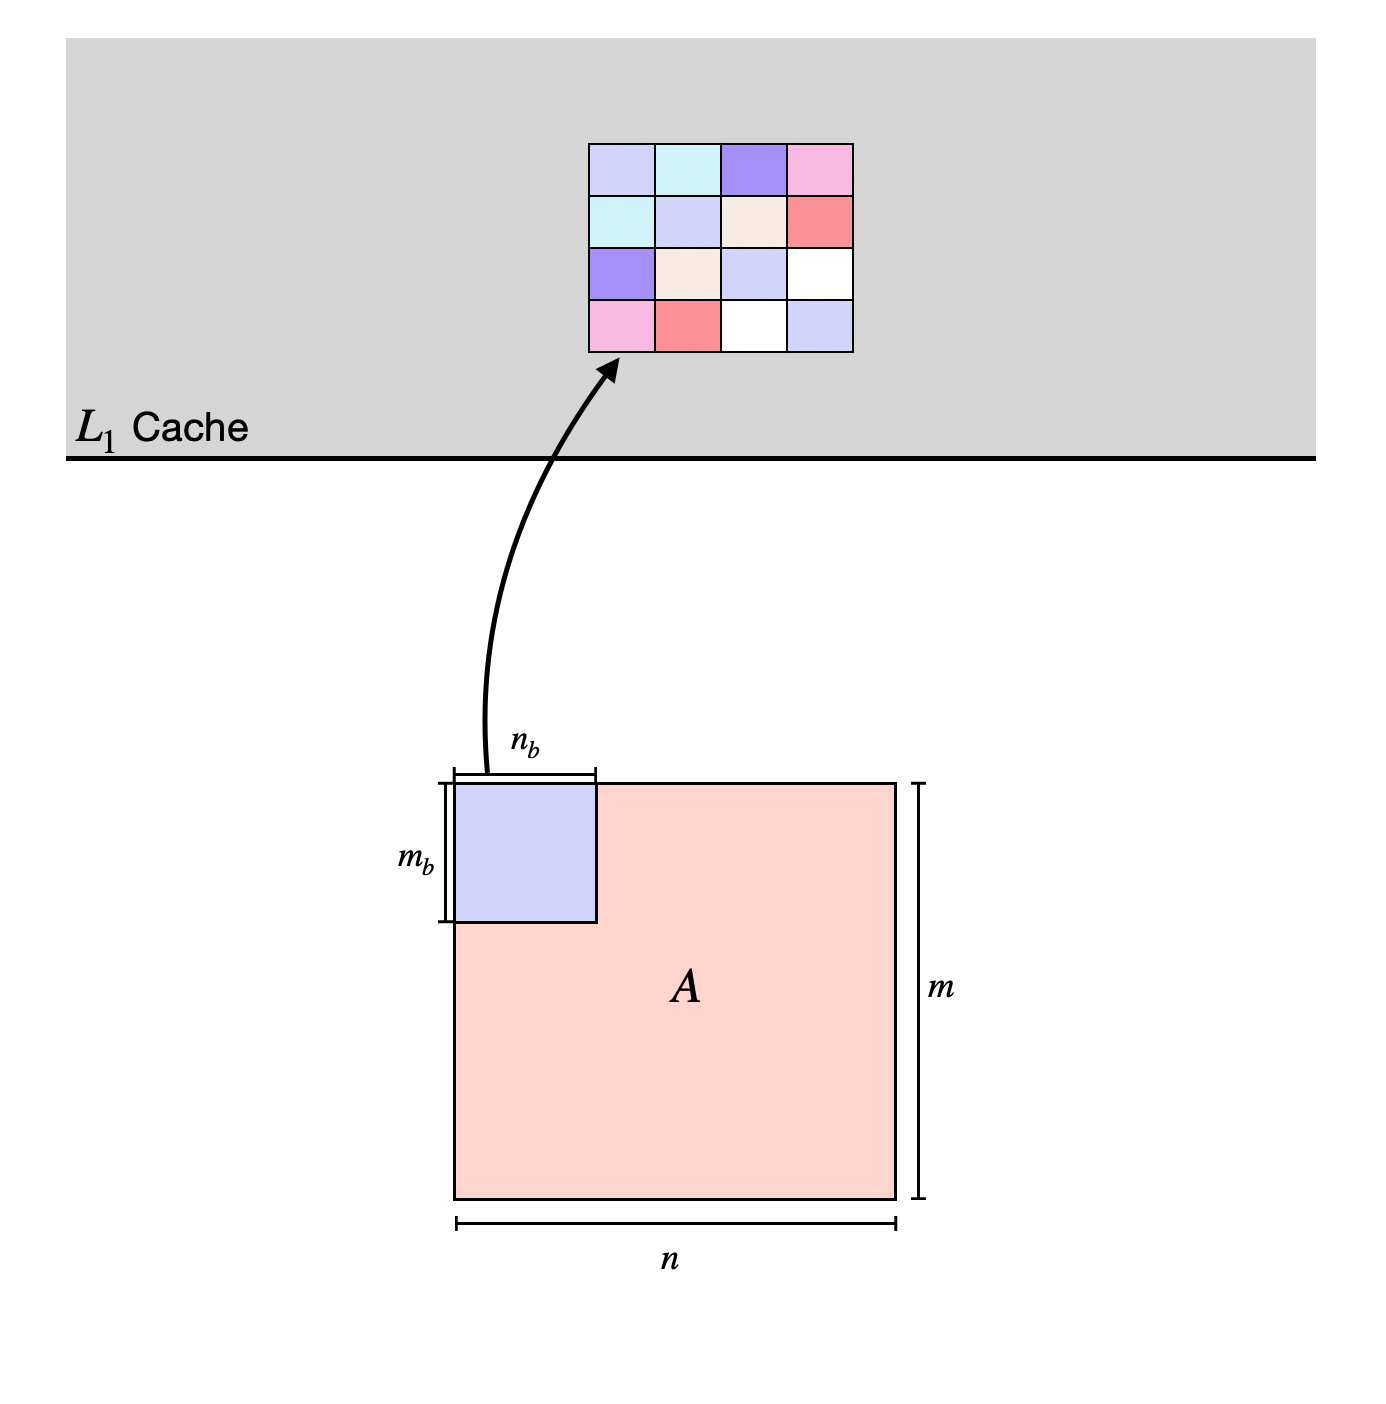
\includegraphics[width=8cm]{../assets/transpose/inplace/inplace_trans2.png} }}%
\end{figure}

\begin{algorithm}[H]
    \SetAlgoLined
    \SetKwFunction{SIMDFn}{$simd\_loop$}
    \SetKwProg{Fn}{Function}{:}{end}

    \tcp{$c$    is the pointer to the output Matrix}
    \tcp{$wc$   is the pointer to the strides of the output Matrix}
    \tcp{$a$    is the pointer to the input Matrix $A$}
    \tcp{$wa$   is the pointer to the strides of the input Matrix $A$}
    \tcp{$m$    is the row-block of the Matrix $A$}
    \tcp{$n$    is the col-block of the Matrix $A$}
    \tcp{$is\_same\_block$ tells us if the $c$ and $b$ are pointing at the same block}
    \Fn{\SIMDFn($c$, $wc$, $a$, $wa$, $m$, $n$, $is\_same\_block$)}{

        \For{\assign{i}{0} \KwTo $m$ \KwBy $1$}{
            \assignln{cj}{c + wc[1] \times i}
            \assignln{aj}{a + wa[0] \times i}
            \assignln{idx}{i * is\_same\_block}
            \openmp{simd}
            \For{\assign{i}{idx} \KwTo $n$ \KwBy $1$}{
                $swap(cj[wc[0] \times j], aj [ wa[1] \times j ])$
            }
        }
    }
    \caption{In-Place Matrix Transpose SIMD Function}
\end{algorithm}


\begin{algorithm}[H]
    \SetAlgoLined
    \KwIn{$c$, $n_c$, $w_c$ $a$, $n_a$, $w_a$, $num\_threads$}
    \tcp{$c$    is the pointer to the output Matrix}
    \tcp{$n_c$  is pointer to the dimensions of the output Matrix}
    \tcp{$w_c$  is pointer to the strides of the output Matrix}
    \tcp{$a$    is the pointer to the input Matrix}
    \tcp{$n_a$  is pointer to the dimensions of the output Matrix}
    \tcp{$w_a$  is pointer to the strides of the output Matrix}
    \tcp{$num\_threads$ is the user provided thread count}
    \tcp{$block$ is the block size for the simd loop}

    \Begin{
        \assignln{m}{n_a[0]}
        \assignln{n}{n_a[1]}
        \assignln{max\_blocks}{max( 1, \lfloor \frac{ m }{block} \rfloor )}
        \assignln{max\_threads}{min( max\_blocks, num\_threads )}
        \openmp{parallel for num\_threads(max\_threads) schedule(dynamic)}
        \For{\assign{j}{0} \KwTo $m$ \KwBy $block$}{
            \assignln{ib}{min( m - i, block)}
            \assignln{aj}{a + i \times wa[0]}
            \assignln{cj}{c + i \times wc[1]}
            \For{\assign{i}{0} \KwTo $n$ \KwBy $block$}{
                \assignln{jb}{min( n - i, block)}
                \assignln{ak}{a + j \times wa[1]}
                \assignln{ck}{c + j \times wc[0]}
                $simd\_loop(ck, w_c, ak, w_a, ib, jb, i == j)$
            }
        }
    }

    \caption{In-Place Matrix Transpose}
\end{algorithm}

\section{Tuning Parameter}

Here, we try to keep the block of the output matrix and the input 
matrix in the $L_1$ cache, which is the help the CPU to access the 
block as fast as possible. The transpose operation is a memory-bound 
algorithm; therefore, we do not control the operation. 

Let the column block be $m_b$ and the row block be $n_b$. Therefore, the block occupies
space of $m_b \times n_b \times S_{data}$ in the $L_1$ cache.

\[
    A_{block} = m_b \times n_b \times S_{data}
\]

\[
    C_{block} = (A_{block})^T
\]

\[
    C_{block} = n_b \times m_b \times S_{data}
\]

Now, we need both blocks to be present in the $L_1$, which means block of matrix $A$
and the block matrix $B$ should occupy $A_{block} + C_{block}$.

\begin{align*}
    S_{L_1} &= A_{block} + C_{block}\\
    S_{L_1} &= m_b \times n_b \times S_{data} + n_b \times m_b \times S_{data}\\
    S_{L_1} &= (m_b \times n_b + n_b \times m_b) \times S_{data}\\
    \frac{S_{L_1}}{S_{data}} &= 2 m_b \times n_b \\
    m_b &\times n_b = \frac{S_{L_1}}{2S_{data}}\\
\end{align*}

In order to maximize the bandwidth, we choose a square matrix, 
and the compiler decides which instructions to emit, or we could 
say that if the rows and columns are equivalent in terms of size, 
we get the best possible bandwidth.

Therefore, $m_b = n_b = B$.

\[B^2 = \frac{S_{L_1}}{2S_{data}}\]
\[B = \sqrt{ \frac{S_{L_1}}{2S_{data}} }\]

An astute reader may observe that cache size and data size are the 
power of two for most of the part because the machine's native language is binary.

We can say that $\frac{S_{L_1}}{S_{data}}$ must a function of the power of two and 
let the power be some $k$.

\[\frac{S_{L_1}}{S_{data}} = 2^k\]

Now, after replacing with the power of two we get

\[B = \sqrt{ \frac{2^k}{2} }\]
\[B = \sqrt{ 2^{k - 1} }\]
\[B = 2^{\lfloor \frac{k - 1}{2} \rfloor}  \]

\clearpage

\section{Performance Plots and Speedup Summary For Out-Of-Place}

\begin{figure}[htb]
    \centering
    \caption*{Performance measurements of transpose implementations}
    \subfloat[\centering Single-Precision]{{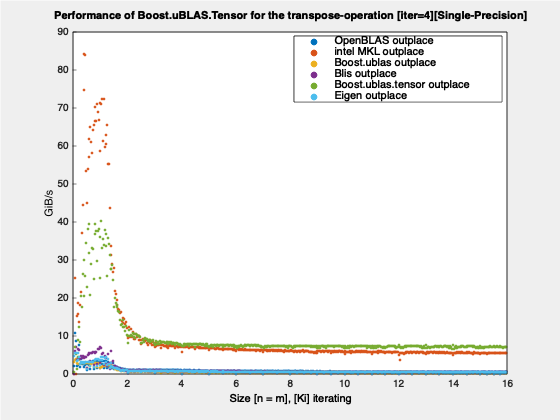
\includegraphics[width=8cm]{../assets/transpose/outplace/float_GiBsVsSize.png} }}%
    \label{fig:trans_outplace_Sgibs220}
    \qquad
    \subfloat[\centering Double-Precision]{{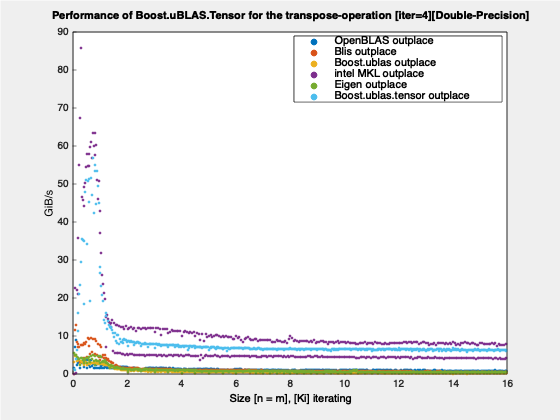
\includegraphics[width=8cm]{../assets/transpose/outplace/double_GiBsVsSize.png} }}%
    \label{fig:trans_outplace_Dgibs220}
\end{figure}

\begin{figure}[htb]
    \centering
    \caption*{Sorted performance measurements of transpose implementations}
    \subfloat[\centering Single-Precision]{{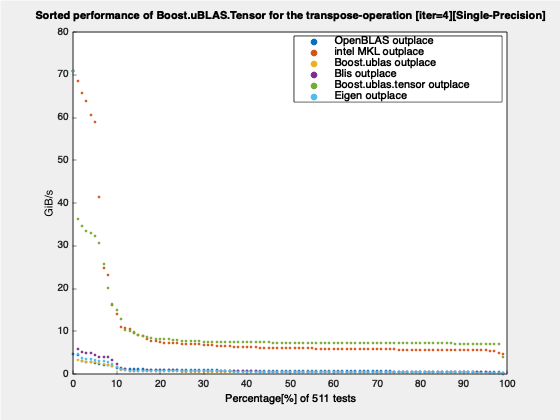
\includegraphics[width=8cm]{../assets/transpose/outplace/float_GiBsVsSize_per.png} }}%
    \label{fig:trans_outplace_Sgibs_per220}
    \qquad
    \subfloat[\centering Double-Precision]{{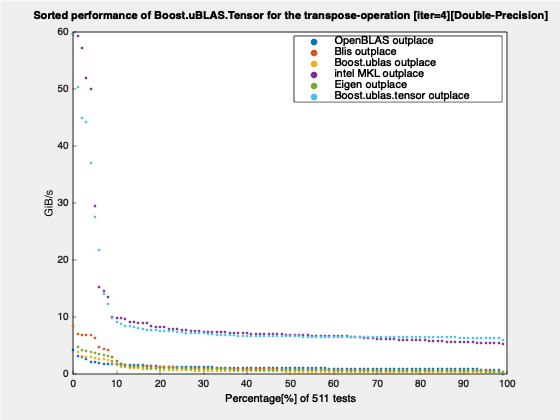
\includegraphics[width=8cm]{../assets/transpose/outplace/double_GiBsVsSize_per.png} }}%
    \label{fig:trans_outplace_Dgibs_per220}
\end{figure}

\begin{figure}[htb]
    \centering
    \caption*{Comparison of the Boost.uBLAS.Tensor transpose implementation}
    \subfloat[\centering Single-Precision]{{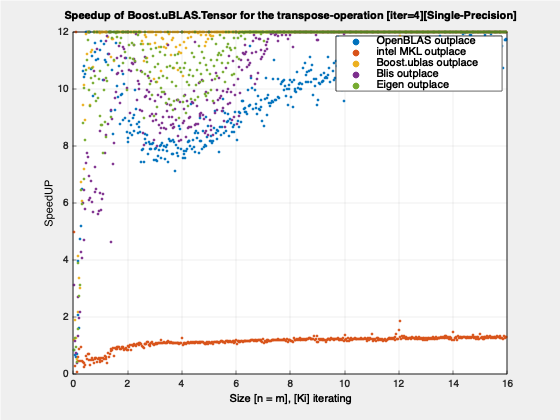
\includegraphics[width=8cm]{../assets/transpose/outplace/float_Speedup.png} }}%
    \label{fig:trans_outplace_Sspeedup220}
    \qquad
    \subfloat[\centering Double-Precision]{{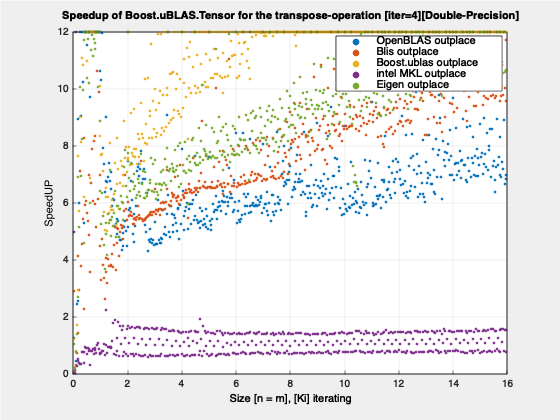
\includegraphics[width=8cm]{../assets/transpose/outplace/double_Speedup.png} }}%
    \label{fig:trans_outplace_Dspeedup220}
\end{figure}

\begin{figure}[htb]
    \centering
    \caption*{Comparison of the Boost.uBLAS.Tensor transpose implementation [sorted]}
    \subfloat[\centering Single-Precision]{{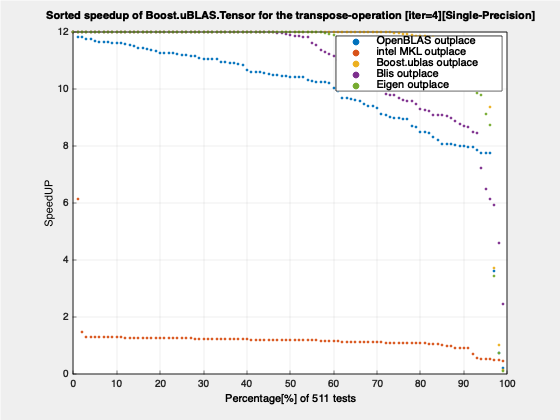
\includegraphics[width=8cm]{../assets/transpose/outplace/float_Speedup_per.png} }}%
    \label{fig:trans_outplace_Sspeedup_per220}
    \qquad
    \subfloat[\centering Double-Precision]{{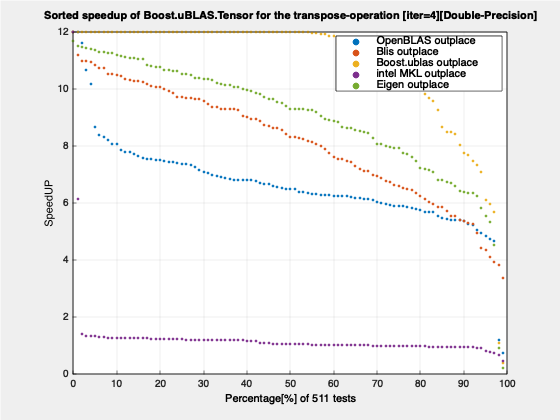
\includegraphics[width=8cm]{../assets/transpose/outplace/double_Speedup_per.png} }}%
    \label{fig:trans_outplace_Dspeedup_per220}
\end{figure}

\begin{table}[ht]
    \centering
    \caption{Speedup Summary For Single-Precision}
    \begin{tabular}{|l|c|c|}
        \hline
        \textbf{Implementation} & \textbf{Speedup $\geq$ 1 [\%]} & \textbf{Speedup $\geq$ 2 [\%]}\\
        \hline
        Boost.uBLAS & $98$ & $97$ \\
        \hline
        OpenBLAS    & $97$ & $97$ \\
        \hline
        Eigen       & $97$ & $97$ \\
        \hline
        Blis        & $99$ & $99$ \\
        \hline
        Intel's MKL & $86$ & $1$ \\
        \hline
    \end{tabular}
    
    \begin{tabular}{|l|c|c|}
        \hline
        \textbf{Implementation} & \textbf{Speed-down $\geq$ 1 [\%]} & \textbf{Speed-down $\geq$ 2 [\%]}\\
        \hline
        Boost.uBLAS & $0$ & $0$ \\
        \hline
        OpenBLAS    & $1$ & $0$ \\
        \hline
        Eigen       & $1$ & $0$ \\
        \hline
        Blis        & $0$ & $0$ \\
        \hline
        Intel's MKL & $12$ & $1$ \\
        \hline
    \end{tabular}
    
    \vspace*{1 cm}

    \centering
    \caption{Speedup Summary For Double-Precision}
    \begin{tabular}{|l|c|c|}
        \hline
        \textbf{Implementation} & \textbf{Speedup $\geq$ 1 [\%]} & \textbf{Speedup $\geq$ 2 [\%]}\\
        \hline
        Boost.uBLAS & $98$ & $97$ \\
        \hline
        OpenBLAS    & $98$ & $97$ \\
        \hline
        Eigen       & $97$ & $97$ \\
        \hline
        Blis        & $99$ & $99$ \\
        \hline
        Intel's MKL & $71$ & $1$ \\
        \hline
    \end{tabular}
    
    \begin{tabular}{|l|c|c|}
        \hline
        \textbf{Implementation} & \textbf{Speed-down $\geq$ 1 [\%]} & \textbf{Speed-down $\geq$ 2 [\%]}\\
        \hline
        Boost.uBLAS & $0$ & $0$ \\
        \hline
        OpenBLAS    & $0$ & $0$ \\
        \hline
        Eigen       & $0$ & $0$ \\
        \hline
        Blis        & $1$ & $0$ \\
        \hline
        Intel's MKL & $27$ & $0$ \\
        \hline
    \end{tabular}
\end{table}

\clearpage
\subsection*{Range[Start: $32$, End: $16Ki$, Step: $32$]}

\begin{table}[ht]
    \centering
    \caption{GiBs For Single-Precision}
    \begin{tabular}{|l|c|c|}
        \hline
        \textbf{Implementation} & \textbf{Max} & \textbf{Average}\\
        \hline
        Boost.uBLAS         & $4.09509$& $0.680433$ \\
        \hline
        Boost.uBLAS.Tensor  & $40.1745$& $9.58504$ \\
        \hline
        Intel's MKL         & $84.1344$& $10.7844$ \\
        \hline
        OpenBLAS            & $10.919$& $0.99106$ \\
        \hline
        Blis                & $7.17433$& $1.00462$ \\
        \hline
        Eigen               & $5.65426$& $0.836292$ \\
        \hline
    \end{tabular}

    \vspace*{1 cm}

    \centering
    \caption{GiBs For Double-Precision}
    \begin{tabular}{|l|c|c|}
        \hline
        \textbf{Implementation} & \textbf{Max} & \textbf{Average}\\
        \hline
        Boost.uBLAS         & $4.98701$& $0.762708$ \\
        \hline
        Boost.uBLAS.Tensor  & $56.7747$& $8.8159$ \\
        \hline
        Intel's MKL         & $85.8162$& $9.80812$ \\
        \hline
        OpenBLAS            & $8.90865$& $1.24028$ \\
        \hline
        Blis                & $13.0382$& $1.34253$ \\
        \hline
        Eigen               & $5.52208$& $1.0204$ \\
        \hline
    \end{tabular}
\end{table}

\begin{table}[ht]
    \centering
    \caption{Speedup(Boost.uBLAS.Tensor) For Single-Precision}
    \begin{tabular}{|l|c|c|}
        \hline
        \textbf{Implementation} & \textbf{Max} & \textbf{Average}\\
        \hline
        Boost.uBLAS         & $9.81041$& $14.0867$ \\
        \hline
        Intel's MKL         & $0.477504$& $0.888787$ \\
        \hline
        OpenBLAS            & $3.67931$& $9.6715$ \\
        \hline
        Blis                & $5.59975$& $9.54096$ \\
        \hline
        Eigen               & $7.10518$& $11.4614$ \\
        \hline
    \end{tabular}

    \vspace*{1 cm}

    \centering
    \caption{Speedup(Boost.uBLAS.Tensor) For Double-Precision}
    \begin{tabular}{|l|c|c|}
        \hline
        \textbf{Implementation} & \textbf{Max} & \textbf{Average}\\
        \hline
        Boost.uBLAS         & $11.3845$& $11.5587$ \\
        \hline
        Intel's MKL         & $0.661585$& $0.898837$ \\
        \hline
        OpenBLAS            & $6.37298$& $7.10797$ \\
        \hline
        Blis                & $4.35447$& $6.56664$ \\
        \hline
        Eigen               & $10.2814$& $8.63965$ \\
        \hline
    \end{tabular}
\end{table}


\clearpage
\section{Performance Plots and Speedup Summary For In-Place}

\begin{figure}[htb]
    \centering
    \caption*{Performance measurements of transpose implementations}
    \subfloat[\centering Single-Precision]{{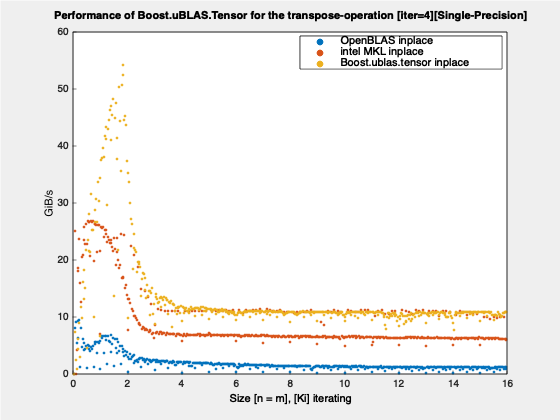
\includegraphics[width=8cm]{../assets/transpose/inplace/float_GiBsVsSize.png} }}%
    \label{fig:trans_inplace_Sgibs220}
    \qquad
    \subfloat[\centering Double-Precision]{{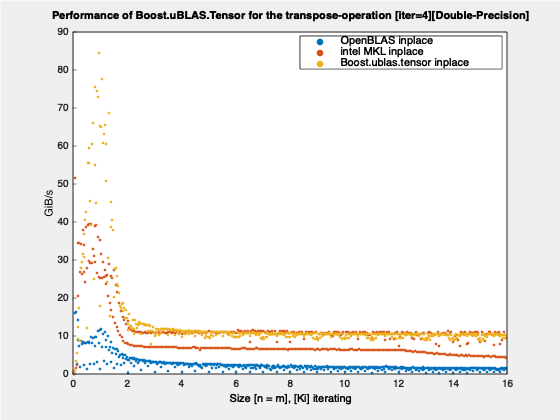
\includegraphics[width=8cm]{../assets/transpose/inplace/double_GiBsVsSize.png} }}%
    \label{fig:trans_inplace_Dgibs220}
\end{figure}

\begin{figure}[htb]
    \centering
    \caption*{Sorted performance measurements of transpose implementations}
    \subfloat[\centering Single-Precision]{{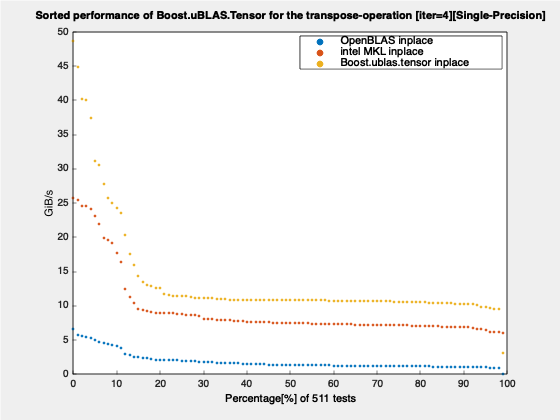
\includegraphics[width=8cm]{../assets/transpose/inplace/float_GiBsVsSize_per.png} }}%
    \label{fig:trans_inplace_Sgibs_per220}
    \qquad
    \subfloat[\centering Double-Precision]{{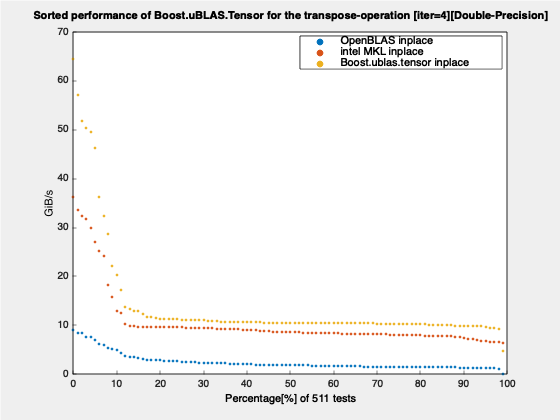
\includegraphics[width=8cm]{../assets/transpose/inplace/double_GiBsVsSize_per.png} }}%
    \label{fig:trans_inplace_Dgibs_per220}
\end{figure}

\begin{figure}[htb]
    \centering
    \caption*{Comparison of the Boost.uBLAS.Tensor transpose implementation}
    \subfloat[\centering Single-Precision]{{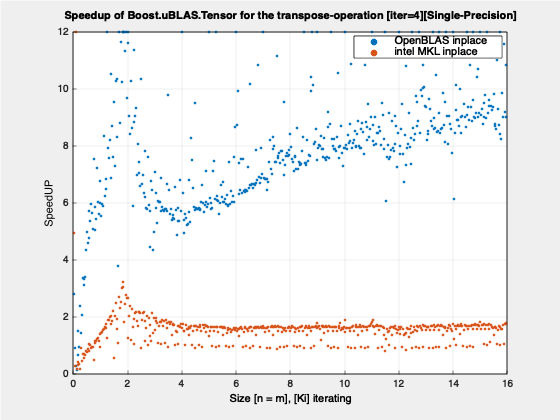
\includegraphics[width=8cm]{../assets/transpose/inplace/float_Speedup.png} }}%
    \label{fig:trans_inplace_Sspeedup220}
    \qquad
    \subfloat[\centering Double-Precision]{{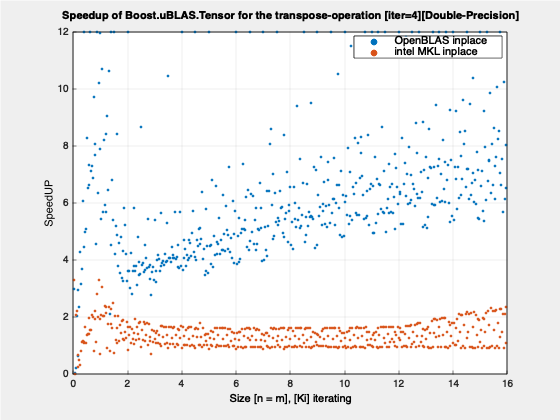
\includegraphics[width=8cm]{../assets/transpose/inplace/double_Speedup.png} }}%
    \label{fig:trans_inplace_Dspeedup220}
\end{figure}

\begin{figure}[htb]
    \centering
    \caption*{Comparison of the Boost.uBLAS.Tensor transpose implementation [sorted]}
    \subfloat[\centering Single-Precision]{{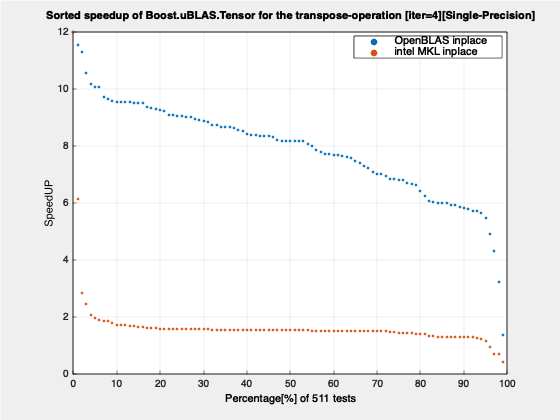
\includegraphics[width=8cm]{../assets/transpose/inplace/float_Speedup_per.png} }}%
    \label{fig:trans_inplace_Sspeedup_per220}
    \qquad
    \subfloat[\centering Double-Precision]{{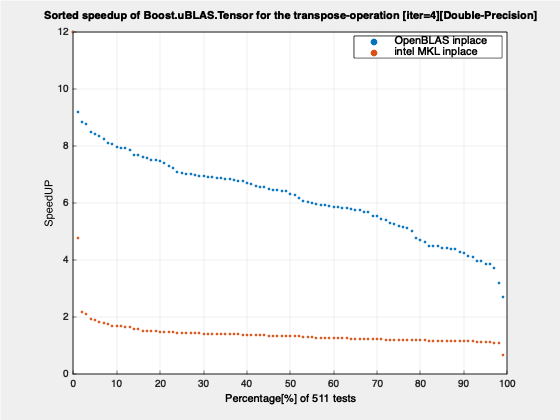
\includegraphics[width=8cm]{../assets/transpose/inplace/double_Speedup_per.png} }}%
    \label{fig:trans_inplace_Dspeedup_per220}
\end{figure}

\begin{table}[ht]
    \centering
    \caption{Speedup Summary For Single-Precision}
    \begin{tabular}{|l|c|c|}
        \hline
        \textbf{Implementation} & \textbf{Speedup $\geq$ 1 [\%]} & \textbf{Speedup $\geq$ 2 [\%]}\\
        \hline
        OpenBLAS    & $99$ & $98$ \\
        \hline
        Intel's MKL & $95$ & $4$ \\
        \hline
    \end{tabular}
    
    \begin{tabular}{|l|c|c|}
        \hline
        \textbf{Implementation} & \textbf{Speed-down $\geq$ 1 [\%]} & \textbf{Speed-down $\geq$ 2 [\%]}\\
        \hline
        OpenBLAS    & $0$ & $0$ \\
        \hline
        Intel's MKL & $3$ & $0$ \\
        \hline
    \end{tabular}
    
    \vspace*{1 cm}

    \centering
    \caption{Speedup Summary For Double-Precision}
    \begin{tabular}{|l|c|c|}
        \hline
        \textbf{Implementation} & \textbf{Speedup $\geq$ 1 [\%]} & \textbf{Speedup $\geq$ 2 [\%]}\\
        \hline
        OpenBLAS    & $99$ & $99$ \\
        \hline
        Intel's MKL & $98$ & $3$ \\
        \hline
    \end{tabular}
    
    \begin{tabular}{|l|c|c|}
        \hline
        \textbf{Implementation} & \textbf{Speed-down $\geq$ 1 [\%]} & \textbf{Speed-down $\geq$ 2 [\%]}\\
        \hline
        OpenBLAS    & $0$ & $0$ \\
        \hline
        Intel's MKL & $0$ & $0$ \\
        \hline
    \end{tabular}
\end{table}


\clearpage
\subsection*{Range[Start: $32$, End: $16Ki$, Step: $32$]}

\begin{table}[ht]
    \centering
    \caption{GiBs For Single-Precision}
    \begin{tabular}{|l|c|c|}
        \hline
        \textbf{Implementation} & \textbf{Max} & \textbf{Average}\\
        \hline
        Boost.uBLAS.Tensor  & $54.1773$& $13.5745$ \\
        \hline
        Intel's MKL         & $26.9047$& $9.3994$ \\
        \hline
        OpenBLAS            & $9.53067$& $1.89466$ \\
        \hline
    \end{tabular}

    \vspace*{1 cm}

    \centering
    \caption{GiBs For Double-Precision}
    \begin{tabular}{|l|c|c|}
        \hline
        \textbf{Implementation} & \textbf{Max} & \textbf{Average}\\
        \hline
        Boost.uBLAS.Tensor  & $84.4904$& $13.7677$ \\
        \hline
        Intel's MKL         & $51.6235$& $10.5006$ \\
        \hline
        OpenBLAS            & $16.47$& $2.51434$ \\
        \hline
    \end{tabular}
\end{table}

\begin{table}[ht]
    \centering
    \caption{Speedup(Boost.uBLAS.Tensor) For Single-Precision}
    \begin{tabular}{|l|c|c|}
        \hline
        \textbf{Implementation} & \textbf{Max} & \textbf{Average}\\
        \hline
        Intel's MKL         & $2.01367$& $1.44419$ \\
        \hline
        OpenBLAS            & $5.68452$& $7.16462$ \\
        \hline
    \end{tabular}

    \vspace*{1 cm}

    \centering
    \caption{Speedup(Boost.uBLAS.Tensor) For Double-Precision}
    \begin{tabular}{|l|c|c|}
        \hline
        \textbf{Implementation} & \textbf{Max} & \textbf{Average}\\
        \hline
        Intel's MKL         & $1.63667$& $1.31113$ \\
        \hline
        OpenBLAS            & $5.12995$& $5.47565$ \\
        \hline
    \end{tabular}
\end{table}